\documentclass[12pt]{article}
\usepackage{graphicx}
\usepackage{wrapfig}
\usepackage{subfigure}
\usepackage{multirow}
\usepackage{hyperref}
\usepackage{amsmath}
\usepackage{amssymb}
\usepackage{ngerman}
\usepackage[ansinew]{inputenc}
\usepackage[left=2cm,top=1cm]{geometry}

% vector graphics test
\usepackage{color}
\usepackage{transparent}
\graphicspath{{graphs/}}





\begin{document}
	\pagestyle{empty}
	\textasciitilde

\begin{titlepage}
    \centering
	\huge{Astronomisches Praktikum: Die Hubble-Konstante}\\
	\bigskip
    \large{Versuch 3}\\
    \huge{Jan R\"{o}der \& Julia Lienert}
\end{titlepage}

%headline!!!


\tableofcontents
\pagebreak

\section{Einleitung}

\section{Methoden zur Entfernungsbestimmung}
\subsection{Cepheidenmethode}
Cepheiden sind Sterne, die ihre Helligkeit periodisch �ndern. Durch Beobachtung der Periode kann �ber die Perioden-Leuchtkraft-Beziehung
\begin{equation}
	M = -2.81 \log\left(\frac{P}{\text{Tage}}\right) -1.43
\end{equation}
auf die absolute Helligkeit geschlossen werden. Zusammen mit der scheinbaren (beobachteten) Helligkeit l�sst sich der Abstand �ber das Entfernungsmodul berechnen.
\begin{equation}
	m - M = 5 \log\left(\frac{r}{10\,\text{pc}}\right)
\end{equation}
Diese Methode ist bis zu einigen Megaparsec anwendbar. Mit dem Hubble-Space-Telescope k�nnen sogar Sterne in bis zu $20 \,$Mpc Entfernung beobachtet und vermessen werden, was eine Beobachtung auch in benachbarten Galaxien m�glich macht.
 
\subsection{Parallaxenmethode}
Bei dieser Methode wird die scheinbare Bewegung naher Sterne vor einem Fixsternhintergrund weit entfernter Sterne gemessen. Sie kommt dadurch zustande, dass sich die Erde im Lauf eines Jahres um die Sonne bewegt. \\
Gemessen wird - wie in Abbildung \ref{fig:Parallaxe} zu sehen ist - der sogenannte Parallaxenwinkel. �ber einfache Geometrie kann dann der Abstand des Sterns berechnet werden. Dazu muss der Abstand von der Erde zur Sonne bekannt sein (verwendet wird hierf�r der mittlere Kreisbahnradius von $1 \,$AE).
\begin{figure}
	\centering
	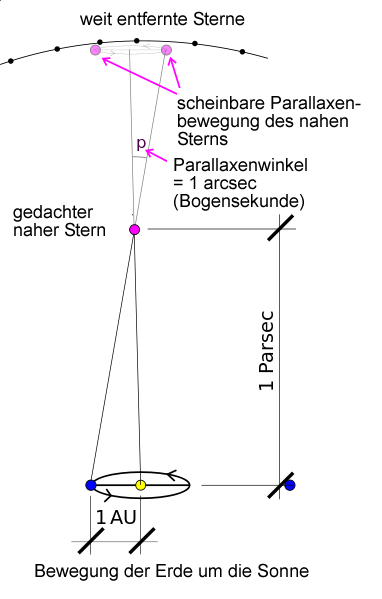
\includegraphics[width=0.5\textwidth]{Parallaxe.png}
	\caption{Skizze zur Erkl�rung der Parallaxe (entnommen aus [1])}
	\label{fig:Parallaxe}
\end{figure}
Entspricht der Parallaxenwinkel genau einer Bogensekunde, so wird die damit verkn�pfte Entfernung als $1 \,$pc bezeichnet. \\
Die Parallaxenmethode kann bis etwa $5000 \,$pc verwendet werden, wenn der Winkel mit dem Hubble-Space-Telescope gemessen wird.

\subsection{Supernova Typ 1a}
Da Supernovae vom Typ 1a immer gleiche Verl�ufe ihrer Lichtkurven haben, k�nnen sie - wie die Cepheiden - als Standardkerzen verwendet werden. Durch Aufnahme der Lichtkurve und Eichung auf eine Lichtkurve bekannten Abstands l�sst sich die Entfernung bestimmen. \\
Diese Methode hat eine Reichweite von �ber $1000 \,$Mpc, da Supernovae diesen Typs sehr leuchtkr�ftig sind.

\subsection{title}






\section{Quellen}
\begin{enumerate}
	\item $https://de.wikipedia.org/wiki/Parallaxe$
\end{enumerate}



\end{document}